\subsection{Energy transported by gravitational wave}

When sources produce gravitational waves, their energy is converted to Gravitational waves. Since generally the sources are very massive Energy of gravitational waves will be very large. Since gravitational wave travels in the speed of light, the energy is also transported at that speed. And since Energy flux is equal to the product of Energy and speed, The average energy flux `$E$' is given by

\begin{equation}
    E = \frac{c^{3}}{16\pi G} \left \langle (h_{+})^{2} + (h_{\times})^{2} \right \rangle 
\end{equation}

So we see the energy flux is very huge because of the term $\frac{c^{3}}{16 \pi G}$ which is in the order of $10^{33}$ Joules sec/ metre$^2$  and it also depends on the average of the square of the plus and cross polarized amplitudes `$h_{+}$' and `$h_{\times}$'. \\

Due to such huge energy it carries the wave can travel unimpeded forever through space and no obstacle can damp gravitational wave because the space in which the obstacle lies itself is the medium of the wave. But the Doppler effect and decrease in amplitude due to radiation of energy causes the wave to die out after the wave travels a very long distance according to the relation $Amplitude \propto \frac{1}{r}$\:. 
\\

\noindent So the power or intensity of gravitational wave decreases as it moves through space according to this inverse square law i.e. as the wave moves in space through a distance `$r$' The energy of wave will be spread-out in space across a sphere of radius`$r$' through Surface area of sphere $4\pi r^2$. Since the intensity of wave is Energy over time, Intensity reduces as $r^2$

\begin{equation*}
    E_{flux}= \frac{Energy}{Area} = \frac{E}{4\pi r^2}
\end{equation*}

\begin{equation*}
    E_{flux} \propto \frac{1}{r^2}
\end{equation*}

\noindent But since $E_{flux} \propto Amplitude^2$ we get the relation that $Amplitude \propto \frac{1}{r}$. i.e Amplitude decreases as distance from source increases. 

\begin{figure}[h]
    \centering
    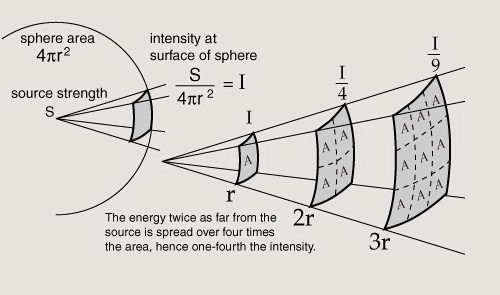
\includegraphics[scale=1]{images.tex/inverse_square.jpeg}
    \caption{ Here we see how the intensity of wave changes as it goes farther from the source according to the inverse square law.\\
    \textbf{Source :-} \url{http://www.mysearch.org.uk/website1/html/339.Laws.html}}
\end{figure}

\pagebreak